\chapter{Experiments}
\label{sec:chapterlabel4}

In the previous chapter, deep reinforcement learning agents were described to solve the recommendation task. Now, in order to test and evaluate their performance, a simulated environment for Recommender Systems is going be defined. Then, after defining the baseline models and the experimental settings, two sets of experiments are carried out: (i) a performance evaluation of the proposed deep learning models and a pure Collaborative Filtering baseline model; and (ii) an analysis of the convergence and speed-up between the deep reinforcement learning agent based on previous work in the area, and an DRL agent with the new policy approach. Final conclusions on the experimental results obtained will be presented in the next chapter.

\section{Reinforcement Learning Environment}

For the purpose to demonstrate how the deep reinforcement learning agent perform on the recommendation task, a simulated environment is modelled under the OpenAI Gym\footnote{\url{https://gym.openai.com/}} reinforcement learning toolkit. It that allow us to define Partially Observed MDP environments (POMDPs)  under an episodic setting where the agent's experience is broken down into a series of episodes \cite{brockman2016openai}. In general, OpenAI Gym manages two core concepts: (1) a free-to-code \textit{agent} that maximizes the convenience for users allowing them to implementation different styles of agent interface; and (2) a common \textit{environment} and action/observation interfaces that ease the implementation and testing of different reinforcement learning problems under the same framework. The final goal in OpenAI Gym is to maximize the expectation of total reward per episode, and to achieve a high level of performance in as few episodes as possible.

During each episode, the agent's initial state is randomly sampled from a distribution, and the interaction proceeds until the environment reaches a terminal state. After performing an action step, the environment interface returns the observation of current state, the reward achieved by the action performed, a done flag indicating if an episode ends and an information object containing useful information for debugging and learning. Finally, the framework also allow us to measure the performance of a RL algorithm under an environment along two axes: \textit{final performance} or average reward per episode, after learning is complete; and, \textit{sample complexity} or the amount of time it takes to learn. 

\subsection{Recommender System Environment}

The recommender system environment, characterized by a set of \textit{n} items to recommend to \textit{m} users, is defined (based on a previous definition in \cite{Dulac-Arnold2015}) as a sequence of MDPs $\langle \mathcal{A}, \mathcal{S}, r, \mathcal{P} \rangle$ composed by an action set $\mathcal{A}$ that correspond to set of items to recommend, a state space $\mathcal{S}$ holding the item the user is currently consuming, a reward $r$ defined as the rating value given by a user to an item if she accepts it, and a transition probability matrix $\mathcal{W}$ which defines the probability of that a user will accept item \textit{j} given that the last item she accepted was item \textit{i}. 

The transition probability matrix is generated using the ideas exposed by Yildirim et al. in \cite{yildirim2008random} to build a random walk recommender system using a Markov Chain mode,l where the probability of being in a state only depends on the previous step $Pr(X_{u, k+1} = i | X_{u, k})$. The algorithm presented in Appendix \ref{app:trans_prob_alg} details the underlying process to set up the environment.

\subsection {Simulation algorithm}

The implemented algorithm is presented in Appendix \ref{app:simulated_env} and describes the complete simulation process of the recommendation task. At each time-step, the agent presents an item \textit{i} to the user with action $\mathcal{A}_i$. The user then accepts the item according to the transition probability matrix $\mathcal{P}$ or selects a random item. To simulate the user patience in a session as in \cite{Dulac-Arnold2015}, an episode of learning ends with probability 0.1 if the user accepts the item, and with probability 0.2 if a random item is selected instead. Finally, after each episode the environment is reset by selecting a random item from a likely subset for an specific user provided by a single item-based collaborative filtering model based on the similarity between items.

\section{Data Set}

The 100-k and 1M Movielens datasets \cite{harper2016movielens} from the GroupLens Reseach Lab\footnote{\url{http://grouplens.org/datasets/movielens/}} are used to train and test the implemented deep reinforcement agents. Table \ref{table:dataset} summarizes the statistical properties of each dataset. The ratings files were pre-processed in order to generate the user rating matrix and the transition probability matrix. Additionally, train and test sets were generated to apply a five-fold cross validation to the baseline CF ratings predictor in the simulated environment.

\begin{table}[!htbp]
%\begin{center}
\centering
\begin{tabular}{ |l|r|r| }
  \hline
%  \multicolumn{2}{|c|}{100K Movielens} & 1M Movielens \\
  & 100K Movielens & 1M Movielens \\
  \hline
  Total ratings & 100,000 & 1,000,029 \\
  Users & 943 & 6,040 \\
  Movies & 1682 & 3,883 \\
  Density & 0.63 & 0.42 \\
%  Sparsity Level & 57.4\% \\
  Mean ratings/user & 106 & 165 \\
  Min. ratings/user & 20 & 20 \\
  Max. ratings/user & 737 & 2314 \\
  \hline
\end{tabular}
%\end{center}
\caption{Properties of the 100-k and 1M Movielens datasets}
\label{table:dataset}
\end{table}

\section{Evaluation Scheme}

For each model proposed below, we measure the average return obtained by the learning agent over steps, as well as the average precision along user sessions or episodes of learning. Finally, a quantitative and qualitative analysis of the results of each model are compared and contrasted against the performance of a random policy which acts randomly by sampling the next action to perform.

\section{Baselines and Experimental Settings}

To evaluate the strength and accuracy of the deep reinforcement learning model under the recommender system environment, we use two variants of the baseline model described in section \ref{sec:baseline}, and a model using the new policy architecture. These models are:

\begin{itemize}
%\item \textbf{FM-MCMC}: \textit{Factorization Machine with Monte Carlo Markov Chain inference}  uses FM based on the Bayeasian inference with a Gibbs sampling technique that generates the distribution of $\hat{y}$ by sampling the conditional posterior distribution for each model parameter. This model was chosen as the baseline model for comparison as it it outperforms other learning approaches like SGD and ALS, and also because it integrates the regularization parameter into the model, which avoids a time-consuming search for the optimal hyperparameters. The only hyperparameter that remains for MCMC is the initialization of the standard deviation$\sigma$ for the Gibbs sampler.
\item \textbf{DRL-kNN-CB}: the \textit{DRL using Content-based item similarity} model uses the DDPG algorithm with a bag-of-words feature vectors to represent actions and states. The k-nearest neighbours index is then created using the KDtree algorithm \cite{friedman1977algorithm} (with 30 leaf nodes cheked) to find the k-closest set of similar items $\mathcal{A}_k$ from the action estimated by the actor function. Finally, the Wolpertinger policy applies the action in $\mathcal{A}_k$ that yields to the maximum return.
\item \textbf{DRL-kNN-CF}: the \textit{DRL with Item-based similarity} model uses the same policy and learning algorithm as the model described above but it implements an item-to item version of the k-NN algorithm by using the item vector representation from the user rating matrix.
\item \textbf{DRL-FM}: the \textit{DRL with Factorization Machines policy} model replaces the k-NN algorithm from the models previously described with the BPR-FM model to return the Top-K items that can be recommended from a given state. Then, the FM-policy will select the action from the top-K recommendations that yields to the highest Q value in the long term. This model can be considered as a hybrid approach as the DDPG algorithm uses a content-based representation of items to estimate the next action, whereas the FM-policy rank items using the information in the user rating matrix.
\end{itemize}
%
%For the FM models, we use the \textit{fastFM}\footnote{\url{https://github.com/ibayer/fastFM}} library introduced by Bayer I. in \cite{bayer2015fastfm} that offers an efficient python implementationn of the FM learning algorithms including MCMC and BRP-OPT with SGDthe ratings file was transformed to the $SVM^{light}$ representation introduced in \cite{joachims1999making}. 

The hyperparameters and network settings used in the experiments are detailed in Appendix \ref{app:hyperparameter}. The network configuration for the DDPG algorithm in the DRL-kNN-CB and DRL-FM models consist of a fully connected network with two hidden layers of 400 and 300 neurons each. while the DRL-kNN-CF model consists of two hidden layers of 1000 neurons. The input and output of the network are the current state (item previously recommended) and the item that the agents predicts to be the next recommendation, respectively. Therefore, their size depends on the vector representation of items in each model.

For the DRL-kNN-CB model, feature vectors for each item were created using a combination of word embeddings extracted using \textit{word2vec}\footnote{\url{https://radimrehurek.com/gensim/index.html}}, and genre categorization as a binary vector. The final feature vector consists of 119 elements. Whereas, for the DRL-kNN-CF, items representation were extracted from the user rating matrix, so their size are 943 and 6040 elements for the 100-k and 1M datasets respectively.

On the other hand, the network input in the DRL-FM model consists of 119 elements (as it uses the same item representation as the DRL-kNN-CB model). Nevertheless, the output size depends on the binary representation of the action set identifiers. For example, for the 100-k dataset, the output size is 11 as the maximum identifier number (1682: the total number of actions) can be represented using eleven binary digits ($1682_{10} = 11010010010_2$).

To build the proposed policy architectures, we use the \textit{NearestNeighbors} model in the \textit{scikit-learn} library\footnote{\url{http://scikit-learn.org}} to train a k-NN model for the Wolpertinger policy using the KD-Tree algorithm, while for the FM-policy, a Ranking FM model is  trained using the algorithm and default hyperparameter configuration provided in the \textit{Graphlab Create} API\footnote{\url{https://turi.com/products/create/}}. Finally, the DRL models are trained using a value of $k$ that corresponds to the 5\% of the action set size (which yielded to good performance in \cite{Dulac-Arnold2015}).

In order to train and use the FM model, items and the current state respectively are formatted using the $SVM^{light}$ representation introduced in \cite{joachims1999making}. Figure \ref{fig:featurevector} presents an example of the feature vector used by the FM model, where the first $|\mathcal{U}|$ binary indicators variables (blue) represent the active user of a transaction, and the next $|\mathcal{I}|$ binary indicator variables (red) hold the active item. Each feature vector also contains normalized indicator variables (yellow) for all other items the user has ever rated. Finally, the vector contains a variable (green) holding the time when the rating was registered, and another variable containing information of the last item the user has rated before.

\begin{figure}[h]
\centering
\caption{Feature vector representation for the FM model. Source: \textit{Factorization machines} \cite{rendle2010factorization}}
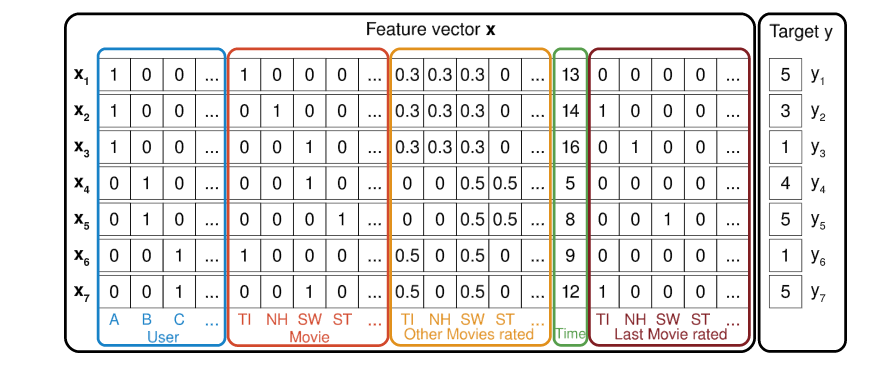
\includegraphics[scale=0.9]{images/featurevectors}
\label{fig:featurevector}
\end{figure}

\section{Results}

The first conducted set of experiments used the 100k Movielens dataset and evaluated the performance of the proposed models after every 100 steps of learning.  Figure \ref{fig:return_train} shows the average return obtained by each agent during learning episodes. It can be seen that our proposed policy architecture outperforms the baselines by obtaining an mean average return of $~ 35$ with an slighty better progression of the performance during 20000 steps, whereas the DRL-kNN-CB model has much less speedup during the first episodes but after 5000 steps it starts to stabilize getting a mean average return of $~ 29$. As a result, the FM-policy is more efficient when finding items that yield to higher rewards than the Wolpertinger policy, evidencing that factorization machine learns latent factors that help to build stronger recommendation models than k-NN.

\begin{figure}[!htbp]
\centering
\caption{Models performance during training in the 100k Movielens recommender task}
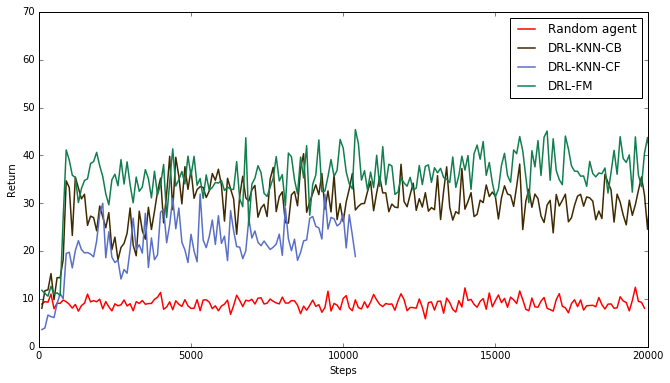
\includegraphics[scale=0.6]{images/eval_return_train}
\label{fig:return_train}
\end{figure}

On the other hand, the DRL-kNN-CF baseline approach does not outperform the content-based model (Its mean average return is $~ 20$), mainly due to the dimensionality of the item representation and consequently the model network size. It also reflects how the representation of the action space affects the behaviour of the k-NN based policy when finding the nearest item that produces the highest reward. Even though the model seems to have a very slow convergence behaviour, it obtains rewards significantly higher that an agent using a random policy.

At the same time, we evaluated the average precision gathered by each model agent over episodes or user sessions. Figure \ref{fig:precision_train} shows that the DRL-kNN-CB model precision fluctuates on values near 0.9, while the DRL-kNN-CF model starts with has lower precision when it starts learning and episodes later it only obtains accuracy values between 0.4 and 0.6. Similarly, the DRL-FM model precision is very low during the first episodes but then it increases sharply and maintains average precision values near one.

\begin{figure}[!htbp]
\centering
\caption{Average precision of recommendations during episodes of learning in the 100k Movielens recommender task}
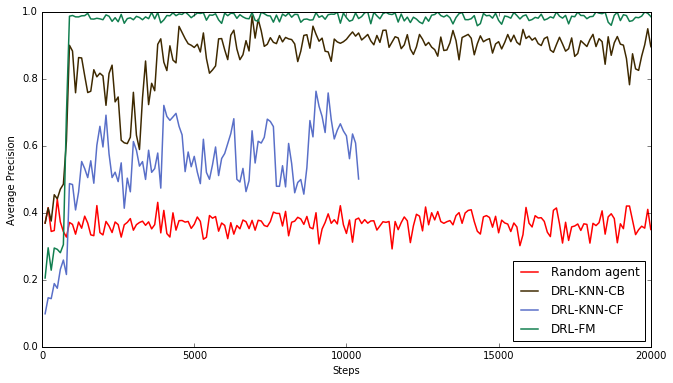
\includegraphics[scale=0.5]{images/eval_precision_train}
\label{fig:precision_train}
\end{figure}

In like manner and with the purpose of demonstrate the importance of the exploration/exploitation trade-off, we test the models by switching off learning (and hence exploration of items)after every 100 steps of training to evaluate how the reinforcement agents act by just exploiting the current learned model parameters. Their behaviour is presented in Figure \ref{fig:return_test} and Figure \ref{fig:precision_test}. As can be seen, the behaviour of the DRL-kNN-CF model and the random policy does not change, but the performance of the DRL-kNN-CB model is approximately similar to the DRL-FM model, obtaining a mean average return of $~34$ and $~ 35$ respectively.

On the other hand, in terms of average precision, both models have episodes when the precision of recommended items lies between 0.9 and 1. Even if it seems to be a good behaviour for an agent, there are certain cases where the same item is recommended more than twice under the same user session. This scenario appears as the simulated environment does not take into account diversity of items being recommended.

\begin{figure}[t]
\centering
\caption{Agent's performance by pure exploitation of the model in the 100k Movielens recommender task}
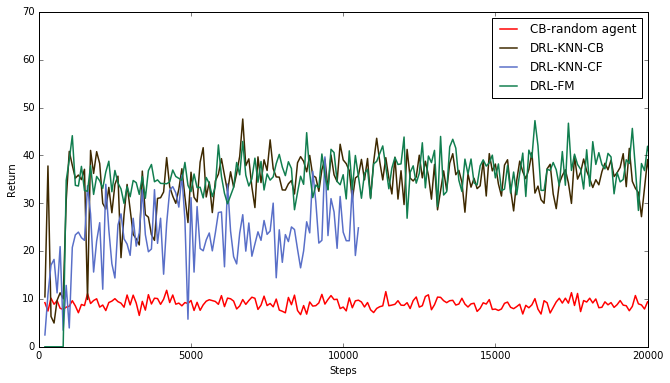
\includegraphics[scale=0.6]{images/eval_return_test}
\label{fig:return_test}
\end{figure}

\begin{figure}[t]
\centering
\caption{Average precision of recommendations by pure exploitation of the model in the 100k Movielens recommender task}
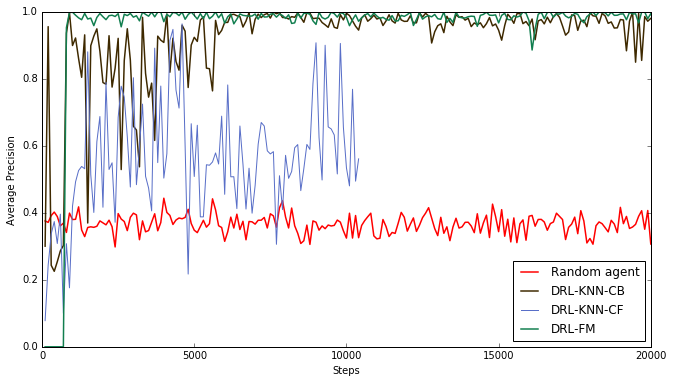
\includegraphics[scale=0.6]{images/eval_precision_test}
\label{fig:precision_test}
\end{figure}